\scanpage{67}
% block: title
\uline{Tannakian categories defined by crystals}.

% block: crystals item 1
\handwritten{1.} Let $k$ be a field of characteristic $p>0$, wh\handwritten{ich} one regards as an algebra over $\underline{Z}_p$, whose maximal ideal is endowed with divided powers. This gives a \unsure{\deleted{e}s|\deleted{s}e}ense to the crystalline site of $k$ (over $\underline{Z}_p$, also q\handwritten{u}alified as ``absolute''), and to the locally free Modules of finite type\inserted{(resp. of finite p\unsure{\deleted{t}r|r|t}esentation)}\handwritten{\begin{tikzpicture}[x=1cm,y=1cm,baseline=-.1cm]\draw[thin] (0,.15).. controls (.05,-.1) and (-.2,-.1)..(-1,-.1)--(-2.1,-.1).. controls (-2.3,-.1) and (-2.35,-.2)..(-2.35,-.5);\end{tikzpicture}} on the latter, which we shall also call crystals in modules (locally free\inserted{resp. of finite presentation}\handwritten{\begin{tikzpicture}[x=1cm,y=1cm,baseline=-.1cm]\draw[thin] (0,.15).. controls (.05,-.1) and (-.2,-.1)..(-1,-.1)--(-2.1,-.1).. controls (-2.3,-.1) and (-2.35,-.2)..(-2.35,-.5);\end{tikzpicture}}) over $k$. These crystals form a $\underline{Z}_p$-linear $\otimes$-category, \deleted{with $\operatorname{Hom}$ which are modules of finite type over $\underline{Z}_p$} One can make this category explicit with the help of a $p$-ring $W$ with residue field $k$, as the category of free modules of finite type (resp. of finite type) $M$ over $\unsure{\mathbb{W}|W}$, with for every integer $n$ an absolute connection on $M_n=M/p^nM$ (relative to 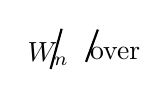
\begin{tikzpicture}[x=1cm,y=1cm,baseline=(w.base)]\node[inner sep=0pt] (w) at (0,0) {$W_n$};\node[inner sep=0pt] at (.85,0) {over};\draw[thick] (.03,-.19)--(.17,.32);\draw[thick] (.48,-.1)--(.63,.31);\end{tikzpicture} $\underline{Z}/p^n\underline{Z}$), of zero curvature, these connections gluing together as $p$ varies. When $\deleted{p}\handwritten{k}$ is perfect, $W$ is the ring of Witt vectors constructed over $k$, and in the preceding description, one can forget the connections: the categories envisaged are simply the category of free modules of finite type (resp. of modules of finite type) over $W$. If $K$ is the field of fractions of $W$, the category of \uline{isocrystals} \deleted{over} (=crystals up to isogeny) over $k$ is equivalent to $\operatorname{Modf}(K)$. \deleted{It is a Tannakian category over $\underline{Q}_p$}

% block: crystals item 2
\handwritten{2.} The category of crystals\unsure{\deleted{n}|n} over $k$ depends functorially on $k$, hence for every crystal the possibility of defining its transform by the base change $\handwritten{\unsure{\sigma|\deleted{\illegible{1}}\sigma}}_k:x\handwritten{\mapsto}x^p:\ k\handwritten{\longrightarrow}k$, say $M^{\handwritten{\unsure{\sigma|\sigma'}}}$. The datum of an $M$ with a hemomorphism
\[
F_M:\ M^{\handwritten{\sigma}}\handwritten{\longrightarrow}M
\]
is called an $F$\handwritten{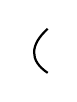
\begin{tikzpicture}[x=1cm,y=1cm,baseline=-.05cm]\draw[thick] (.12,.3).. controls (-.1,.1) and (-.12,-.1)..(.12,-.26);\end{tikzpicture}}-\uline{crystal over} $k$. We shall note that the $F$-crystals form a \inserted{$\underline{Z}_p$-linear}\handwritten{\begin{tikzpicture}[x=1cm,y=1cm,baseline=-.1cm]\draw[thin] (0,.15).. controls (.05,-.1) and (-.2,-.1)..(-1,-.1)--(-2.1,-.1).. controls (-2.3,-.1) and (-2.35,-.2)..(-2.35,-.5);\end{tikzpicture}} \inserted{$\otimes$-}\handwritten{\begin{tikzpicture}[x=1cm,y=1cm,baseline=-.1cm]\draw[thin] (0,.3).. controls (0,0) and (-.5,-.05)..(-.55,-.45);\end{tikzpicture}}category whose $\operatorname{Hom}$ are modules of finite type over $\underline{Z}_p$ (beware, not\inserted{\handwritten{modules}}\handwritten{\begin{tikzpicture}[x=1cm,y=1cm,baseline=-.1cm]\draw[thin] (0,.15).. controls (.05,-.1) and (-.2,-.1)..(-1,-.1)--(-2.1,-.1).. controls (-2.3,-.1) and (-2.35,-.2)..(-2.35,-.5);\end{tikzpicture}} over $W$, even if $k$ is perfect !). This \unsure{\deleted{t}i|\deleted{i}i|i}s not a \deleted{\unsure{category|ctategory}} Tannakian category, even once tensored with $\underline{Q}_p$, for it lack
% archive sheet number: 66
